\section*{Introduction}
The task of inferring the identity of an author from his or her writing style has been studied for many centuries. Aspects such as punctuation, word use, and other stylometric features are used to
to `fingerprint' an author to identify an an anonymous author or to verify the authorship of a disputed work.

Recent advancements in machine learning and language modelling have been exploited to some extent to improve the state of the art of authorship attribution, but there are still many avenues to explore. 
Specifically, while Support Vector Machines, Decision Trees, Clustering, and other machine learning techniques have been applied to the problem, there have only been limited attempts to leverage advances in 
neural networks and deep learning for this task.
Neural network approaches to authorship identification face several challenges. The most noteable of these is arguably the data-scarcity issue: Neural approaches often require substantially more data than other classifiers. When doing authorship identification, there is often very little data available. An authorship verification task, for example, might consist of two texts of a few thousand words each: The author of the first text is known and alleged to be the same as the second text and a classifier should decide whether or not it is plausible for the two texts to share an author.

We propose to investigate whether the challenges related to using neural networks as tools for authorship identification can be overcome.
In response to the data-scarcity issue, we propose combining transfer learning with character-level language modelling, 
as both of these techniques have been used in prior work where data scarcity was an issue. 
We also propose to link research from areas related to authorship identification. 
On a more general level, authorship attribution can be seen as a task of separating \textit{style} from \textit{content}. 
The same author may write on very different topics, but some unique part of the author's style is often still visible. 
In order to effectively identify authors, a classifier needs to look for similarity in style while ignoring differences in content. 
The style/content separation challenge is also found in:

\begin{itemize}
    \item Voice recognition: some systems can recognise who is speaking, regardless of what they say.
    \item Image re-identification: access systems, for example, which take an in initial picture of an authorized person and then need to verify that later photos are the same, ignoring dress and pose.
    \item Artistic style transfer: Recent research has shown that it is possible to transfer the artistic style of an artist (e.g. transforming a modern photo to look as though it was painted in Van Goch's distinctive style).
    \item Plagiarism detection: modern plagiarism detection systems can detect a sudden change in authorship style (even though content remains the same).
    \item Style transfer: some work aims to `translate' content between broader text styles, such as automatically re-generating shakespeare texts in modern, simpler language.
    \item Signature verification: an image of a forged signature has very similar content to a proof signature, and signature verification systems aim to detect the difference in style.
    \item Handwriting style: Generating new handwriting styles for arbitrary text relies on some amount of style and content separation.
\end{itemize}

Outside content and style separation research, there have also been recent advances in specific neural network architectures and in language modelling techniques. 
While most prior research relies on shallow features and simple classifers, modern approaches to many problems rely on deeper features, such as semantic word and character embeddings, and more sophisticated classifiers, containing specialised neural network cells (such as Long-Short term Memory cells, from RNN-LSTM models) or optimized architectures (such as Siamese Neural Networks, where weights are shared between similar inputs, allowing the network to learn a distance function). 

In what follows, we present a review of prior work, looking work directly related to authorship identification and authorship attribution, as well as research that covers indirectly related research, such as language modelling, and the style/content separation discussed above. We further include an overview of open datasets that are commonly used in authorship identification. We then present the exploratory experiments that we have completed so far, and end off with a proposed timeline of how the remaining research will be carried out.


\section*{Literature review}
We present a summary of some of the most important existing research. We begin with research that is directly related to the task at hand (i.e. authorship verification and author identification). We follow this with a section which presents prior research into language modelling, with a focus on character-based RNN-LSTM language models, which are the current state of art for many language tasks. We then present work that has used specialised network architectures, such as siamese networks or networks which make use of transfer learning. 

\citet{stamatatos2009survey} provides the most extensive survey of prior work, covering authorship attribution research between the 19th century and 2009. Stamatatos provides a comprehensive overview of the different classes of features that are useful for authorship attribution as well as an overview of different ways the task can be modelled. 
He breaks features into five broad categories, namely Lexical (e.g. word frequencies), Character (e.g. character n-grams), Syntactic (e.g. Part-of-Speech tags), Semantic (e.g. synonyms), and Application Specific (e.g. structural features). 
We will take special interest in looking for improvements in semantic features, as there have been important advances in NLP in this area, notably the now ubiquitous skip-gram and word2vec algorithms proposed from \cite{mikolov2013efficient} and \cite{mikolov2013distributed} as well as \citep{audhkhasi2017end} who use a CNN to train character-embeddings and then feed these embeddings into a RNN to create a language model. 

Stamatatos also divides authorship attribution methods into two classes: profile-based approaches and instance-based approaches. In the former, we attempt to create a profile or model of each author. 
Texts can then be classified by seeing which author-profile they most closely match. For example, we can train separate generative language models for a number of different authors, and then classify texts based on how closely they fit to specific models.
In the latter, we look at the relation between the texts themselves. For example, we could take a simple cosine distance between two texts, using TF-IDF features, and use this as information to support or reject a hypothesis that the two texts were written by the same person. In our work, we propose to attempt both approaches. We will use RNN-LSTM langauge modelling to attempt profile-based authorship attribution and Siamese Networks to attempt instance-based attribution.

Although we mentioned character-level langauge modelling above with regards to data-scarcity, character-level modelling has other advantages for the authorship attribution task. 
\citep{sapkota2015not} show that character n-grams perform well for authorship tasks mainly because of their ability to capture affixes and punctuation.
Both affixes and punctuation are largely ignored in word-based language models, but many authors use these in highly specific ways. Word models can provide useful information too, however. \citep{kestemont2014function} talks about why function words have generally been regarded as important for authorship attribution.
He also argues that function words are largely only useful in English language settings, and concludes that character-based models are far better at generalizing to other langauges.

Although discriminating between authors based on their personal writing styles is already a challenging task, it is made more difficult when an author deliberately tries to simulate the writing style of another. Arguably the most-admired \textit{Pistache} is ``Alice Through the Needle's Eye'', a word which attempts to copy the writing-style of Lewis Carol's ``Alice in Wonderland''. \citep{somers2003authorship} focus on this work and discuss some basic stylometry features such as lexical richness.

Recently, \citep{bagnall2015author} created a multi-headed character-level recurrent neural network for authorship attribution, and used to to achieve the highest score in the PAN 15 shared task on authorship verification. This work is of special interest to us as it addresses the aforementioned data-scarcity challenge. Bagnall uses data from all authors in the dataset to train author-specific models, which partly mitigates the problem that there is very little data available for each author. This is similar to our proposed approach, where we attempt to train a language model that can learn general-language rules from a larger corpus before `tuning' the model on an author's specific style.

\subsection*{Siamese networks}
Siamese networks are neural networks which learn a distance function between pairs of training examples. They were first introduced by  
\citep{bromley1993signature} who proposed using the architecture for signature verification. They have more recently been used for scene boundary detection (deciding if two film frames are from the same scene), 
\cite{baraldi2015deep} and image re-identification (deciding if two images are of the same person) \cite{zhu2017deep}. There is less research in using siamese networks for language tasks, but notable exceptions are 
\citep{hosseini2015similarity} who use a Siamese network to help with OCR (instead of doing full analysis of handwritten text in an image, they can find similar images that have already been OCRed);
\citep{neculoiu2016learning} who use a Siamese Network to match job titles on similarity (For example, mapping ``software architectural technician Java/J2EE'' to ``Java Engineer''); 
as well as \citep{mueller2016siamese} and \citep{yin2015abcnn} who use siamese networks for sentence similarity tasks. Also related is work by 
\citep{hoffer2015deep} who create a so-called ``Triple Network'', which extends the idea of a Siamese Network. It takes three inputs instead of two -- X, X+ and X-, where X and X+ are the same class and X- is a different class.


\subsection*{Transfer learning and style transfer}
Transfer learning refers to re-using some weights from a previously trained network on a new task. 
\cite{raghu2016expressive} talk about the relation between the structure of a neural network and the functions that it is able to compute. They state that lower layers are more important and are more sensitive to noise and optimizations, while higher layers can model exponentially more complex functions. 
\citep{gatys2015neural} use this to transfer the style of an art image to an image with different content (e.g. making a photograph of your house look as though it was painted by Van Goch.). 
They extract style information from the higher layers of a CNN and content information from the lower layers in order to create a new image with the content of one image and the style of another.

This is strongly related to the content/style separation mentioned before, but it also leads to the idea that we have a small amount of data for a specific task (such as authorship attribution) but a large amount of data for a more general task (e.g. language modelling), then we can improve performance on the specific task by using some knowledge learned during training for the general task. Retraining only specific layers of a network in order to model a new task is used primarily in three settings, namely:

\begin{enumerate}
    \item when there is not enough data available for the specific task, and more information needs to be extracted from a larger and more general dataset -- e.g. \citep{zoph2016transfer} use transfer learning to improve neural machine translation on low-resource language pairs;
    \item when there is a limitation on computational resources at run time, for example \citep{yoon2017efficient} look at transfer learning for training user-specific language models on mobile devices, and 
\cite{mcgraw2016personalized} use an RNN-LSTM for personalized speech recognition on mobile devices;
    \item when there are privacy considerations, and it is important that the network does not `leak' any information from the training data. \citep{shin2016generative} use a `teacher-learner' transfer model, in which the student is trained on the output of the teacher.
\end{enumerate}

Also related to transfer learning is work by 
\citep{lalor2017improving} who talk about the fine-tuning a neural model by adding supplemental data. 
They distinguish this from transfer learning, saying that while transfer learning uses data from a different task, 
fine-tuning re-uses data from the same task.

Although we found no prior research related to transfering \textit{authorship} style from one document to another, there has been some work in transfering \textit{genre} style.
\citep{kabbara2016stylistic}, for example, describe a system that could be trained on Wikipedia and equivilant articles from Simple English Wikipedia. When fed works by Shakespeare, it would aim to produce simplified (or modernized) Shakespeare text. 


\subsection*{Language modelling}

For profile-based authorship attribution methods, generative language models are used. Therefore, research which deals with language modelling in general is relevant to our work.
\citep{karpathy2015unreasonable2} shows how well an RNN can be used to model different styles of language using only characters. For example, when trained on Shakespeare's work, an RNN can generate text 
which at first glance appears to be Shakespeare. When the same network is trained on modern technology essays, it produces text in a completely different style. 
If we can train an algorithm to \textit{generate} text in a specific style, it is easy to adapt this to \textit{recognise} the style a text is written in, which is exactly what we attempt to do for authorship attribution. 


\section*{Exploratory experiments and timeline for future work}
So far, we have conducted some basic exploratory experiments for both author-based and instance-based approaches. For the former, we trained an RNN-LSTM generative language model using two LSTM layers with a size of 256 and dense layer with softmax activation. We used a sequence length of 100 characters. For training data, we used the texts of
\textit{Alice in Wonderland}, 
\textit{Huckleberry Finn}, and 
\textit{Pride and Prejudice} 
We used these to create what we refer to as a generic language model. We then retrained the Dense output layer only for each author in the PAN 2015 authorship verification dataset\footnote{http://pan.webis.de/clef15/pan15-web/author-identification.html} to create what we refer to as a 'tuned' language model for each author.

Each instance in the dataset contains a 'known' text and an 'unknown' text. The task is to predict whether the 'unknown' text is by the same author as the 'known' one. We hypothesised that a language model tuned to a specific author would better model the 'unknown' text for instances where the author was shared than for instances with different authors. Preliminary results suggest that we can achieve a baseline score of about 0.65 accuracy simply by looking at how much better the tuned model performs on a given unknown text and comparing this to how well the generic language model performs. We expect that we can do better than this by improving our generic and tuned language models, and we plan to experiment with using different and/or more training data, as well as trying attempting to optimize the hyperparamters and architecture of the language model.

For the instance-based approach, we trained a Siamese network consisting of two Dense layers of size 128 and ReLu activation. We represent each text as a simple bag of characters, taking only the first 1200 characters of each text as all texts needed to be the same size for the comparison. This network was able to learn a distance function that could get a cross-validated accuracy of over 85 percent for the PAN training dataset. However, this method has so far not proven to be very robust, and testing the model on different datasets performs no better than chance. We expect that our results can be improved by experimenting with different methods of text vectorization, or by using an LSTM Siamese model that can better model sequences of characters.

\begin{figure}[h]
    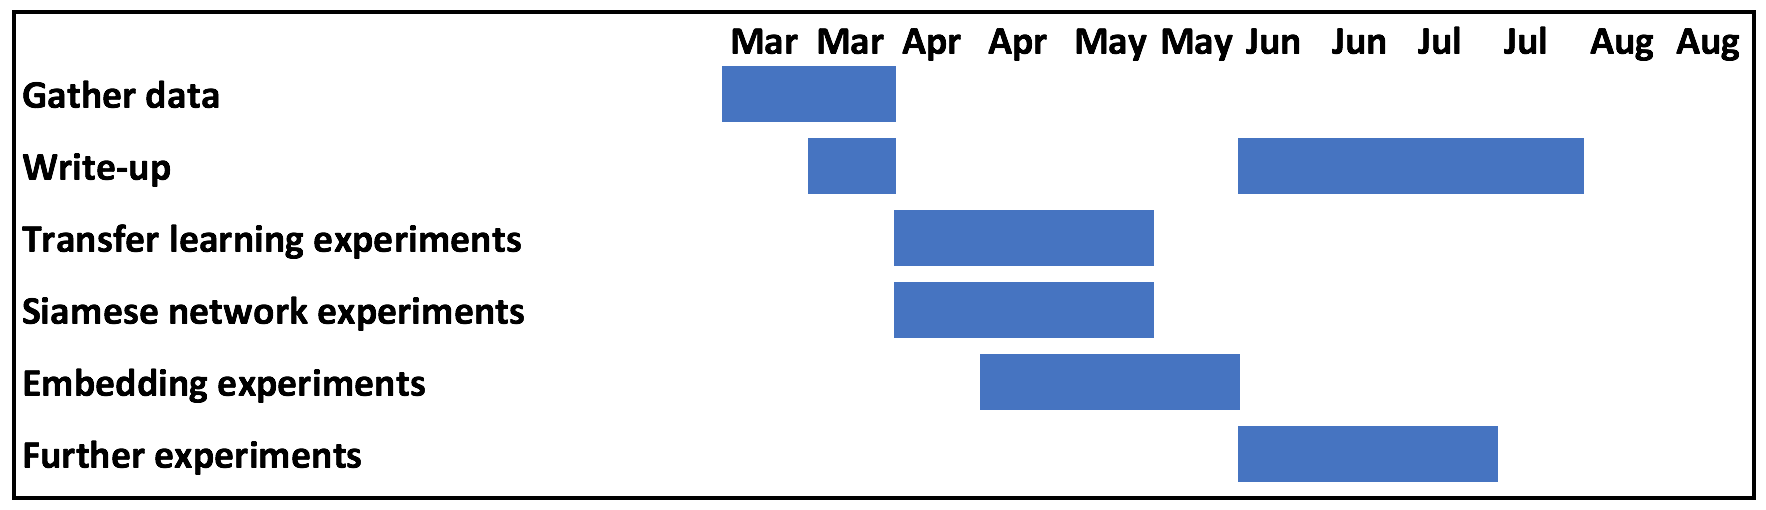
\includegraphics[width=\textwidth]{gantt}
\label{fig:model}
\caption{Proposed timeline for future work. Each month is present twice to indicate the first and second halves of that month. 
``Further experiments'' is time we have reserved for conducting experiments that we expect to design based on the results of the previous experiments. August is reserved for any unexpected delays.}
\end{figure}

We plan to focus our research efforts on a) improving the results discussed above, and b) exploring using word- and/or character embeddings as features, instead of the simple character representations that we have used up to now.

In summary, we propose investigating the following approaches:
\begin{itemize}
    \item Investigate using a character-based RNN-LSTM generative language model with transfer learning for authorship attribution
    \item Investigate using a Siamese architecture for modelling a distance function between two texts, and applying this to authorship verification.
    \item Investigate whether word and/or character embeddings can improve over simpler representations for authorship attribution.
\end{itemize}

The proposed timeline for this research can be seen in the Gantt chart in Figure 1.


